%!TEX root = ../doc.tex
\chapter{Wireless LAN Grundlagen}
\label{sec:TheoretischeGrundlagen}

\section{Definition}
Ein Wireless LAN ist ein Funknetz welches die Übertragung von Daten von einem Endgerät (Computer, Handy, usw.) durch den offenen Raum zu einem Access Point erlaubt. Die meisten Wireless LAN Standards sind in der IEEE-802.11 Familie beschrieben und werden von den meisten neueren Geärten, welche mit Wireless LAN ausgestattet sind, unterstützt. Das Wireless LAN ersetzt in vielen Bereichen das LAN bzw. das Kabel, welches früher für die Verbindung mit einem LAN benötigt wurde.

\section{Technisch}
Die Primäre Funktion eines Wireless LAN Access Point ist das erstellen einer Verbindung zwischen 802.11 Wireless LAN und 802.3 Ethernet Datenverkehr. Ein Access Point auch Router genannt sendet in einem Intervall (ca. 10 mal pro Sekunde) seine Verbindungsinformationen an alle Wireless Geräte in seiner Reichweite. Die Informationen bestehen aus folgenden Bestandteilen.
\begin{itemize}
\item Der Netzwerkname - Service Set Identifier (SSID)
\item Die Liste der unterstützten Übertragungsraten
\item Die Art der Verschlüsselung
\end{itemize}
Mit diesen Angaben kann ein Wireless Gerät mit dem korrekten Passwort sofern notwendig eine Verbindung mit dem Access Point herstellen. Wireless LAN Access Points operieren auf der Sicherungsschicht (Schicht 2) des OSI Modell. Daher verwenden sie die gleiche Adressierung wie herkömmliche LANs und können auch ohne weiteres mit diesen Kommunizieren.

SSID -BSSID


\section{Verbreitung}
Das Schweizer Bundesamt für Statistik hat im Februar 2011 Daten zur Internetnutzung der Schweiz erhoben und kam zum Schluss, dass 58\% der Schweizer Haushalte über ein Wireless LAN verfügen\citep[S. 8]{bfs.internet.2011}. Zusätzlich werden in den grösseren Städten in den öffentlichen Gebäuden (Bahnhof, Flughafen usw.) sowie in vielen Cafes Wireless LANs Gratis oder gegen Bezahlung angeboten. Zahlen zu der Dichte von Wireless LAN in Europäischen Städten scheint es nicht zu geben oder sind sehr schwierig zu Finden. Für die Benutzbarkeit der zu erstellenden App ist das Aufkommen von Wireless LANs in den Städten ein kritischer Faktor.

\subsection{Experiment Zürich}
Um Einschätzen zu können wie viele Access Point in einer Stadt zu finden sind wurde ein kleines Experiment durch geführt. Mit der Android App WiFi Tracker\citep{google.play.wifitracker} werden alle empfangen Wireless LAN Netzwerke mit den aktuellen GPS Koordinaten des Mobiltelefon gespeichert. Mit dem Fahrrad und dem Mobiltelefon wurde eine Strecke von ca. 3.1 Kilometern durch den Zürcher Kreis 4 gefahren. Die Aufgezeichneten Daten bringen erstaunliches zum Vorschein.
\begin{figure}[ht]
	\centering
	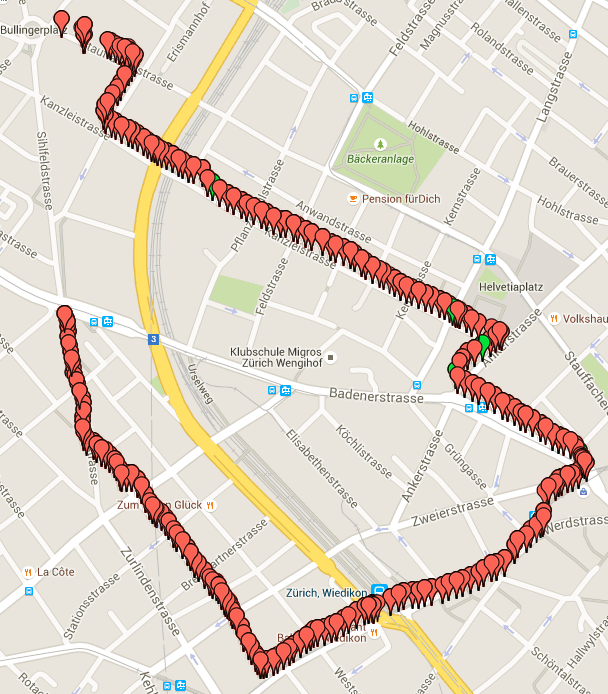
\includegraphics[width=0.8\textwidth]{images/wifikreis4.png}
	\caption{Wireless LANs gemesen mit WiFi Tracker im Zürcher Kreis 4}
	\label{fig:wifikreis4}
\end{figure}
Auf der Strecke wurden 2253 unterschiedliche Access Points gemessen welche in der Abbildung\ref{fig:wifikreis4} visuell dargestellt sind. Das heisst durchschnittlich ist alle 1.37 Meter ein neuer Access Point zu finden. Diese Zahlen müssen natürlich ein wenig relativiert werden da die 2253 Access Points nicht zwingend auch eigene Wireless LAN Netzwerke sind. Wie oben beschrieben können mehrere Access Points mit der selben SSID zu einem Wireless LAN Netzwerk gehören. Zusätzlich ist der Zürcher Kreis 4 nicht ein Gebiet dass auf den Rest von Zürich oder andere Städte schliessen lässt. Trotzdem lassen diese Zahlen auf eine grosse Wireless LAN Dichte in Schweizerischen Städten deuten.


